\documentclass[11pt]{article}

\usepackage{xcolor}
\usepackage{mathtools}
\usepackage[legalpaper, margin=1in]{geometry}
\usepackage{amsmath}
\usepackage{amssymb}
\usepackage{paralist}
\usepackage{enumitem}
\usepackage{rsfso}

\newcommand{\R}{\mathbb{R}}
\newcommand{\N}{\mathbb{N}}
\newcommand{\Z}{\mathbb{Z}}
\newcommand{\Q}{\mathbb{Q}}
\newcommand{\A}{\mathcal{A}}
\newcommand{\J}{\mathcal{J}}
\newcommand{\T}{\mathcal{T}}
\newcommand{\C}{\mathcal{C}}
\newcommand{\M}{\mathcal{M}}
\newcommand{\Complex}{\mathbb{C}}
\newcommand{\Power}{\mathcal{P}}
\newcommand{\note}{\color{gray}Note: \color{black}}
\newcommand{\notation}{\color{gray}Notation: \color{black}}
\newcommand{\fact}{\color{gray}Fact: \color{black}}
\newcommand{\Intab}{[\,a,b\,]}





\begin{document}

	\begin{titlepage}
		\begin{center}
			\topskip0pt
			\vspace*{\fill}
			\Huge \color{red}
				\textbf{Definitions and Notes}\\
			\vspace{0.5cm}			
			\Large \color{black}
				Math 295 - Honors Mathematics I\\
				Professor Sarah Koch\\		
				University of Michigan\\
			\vspace{3cm}
			
			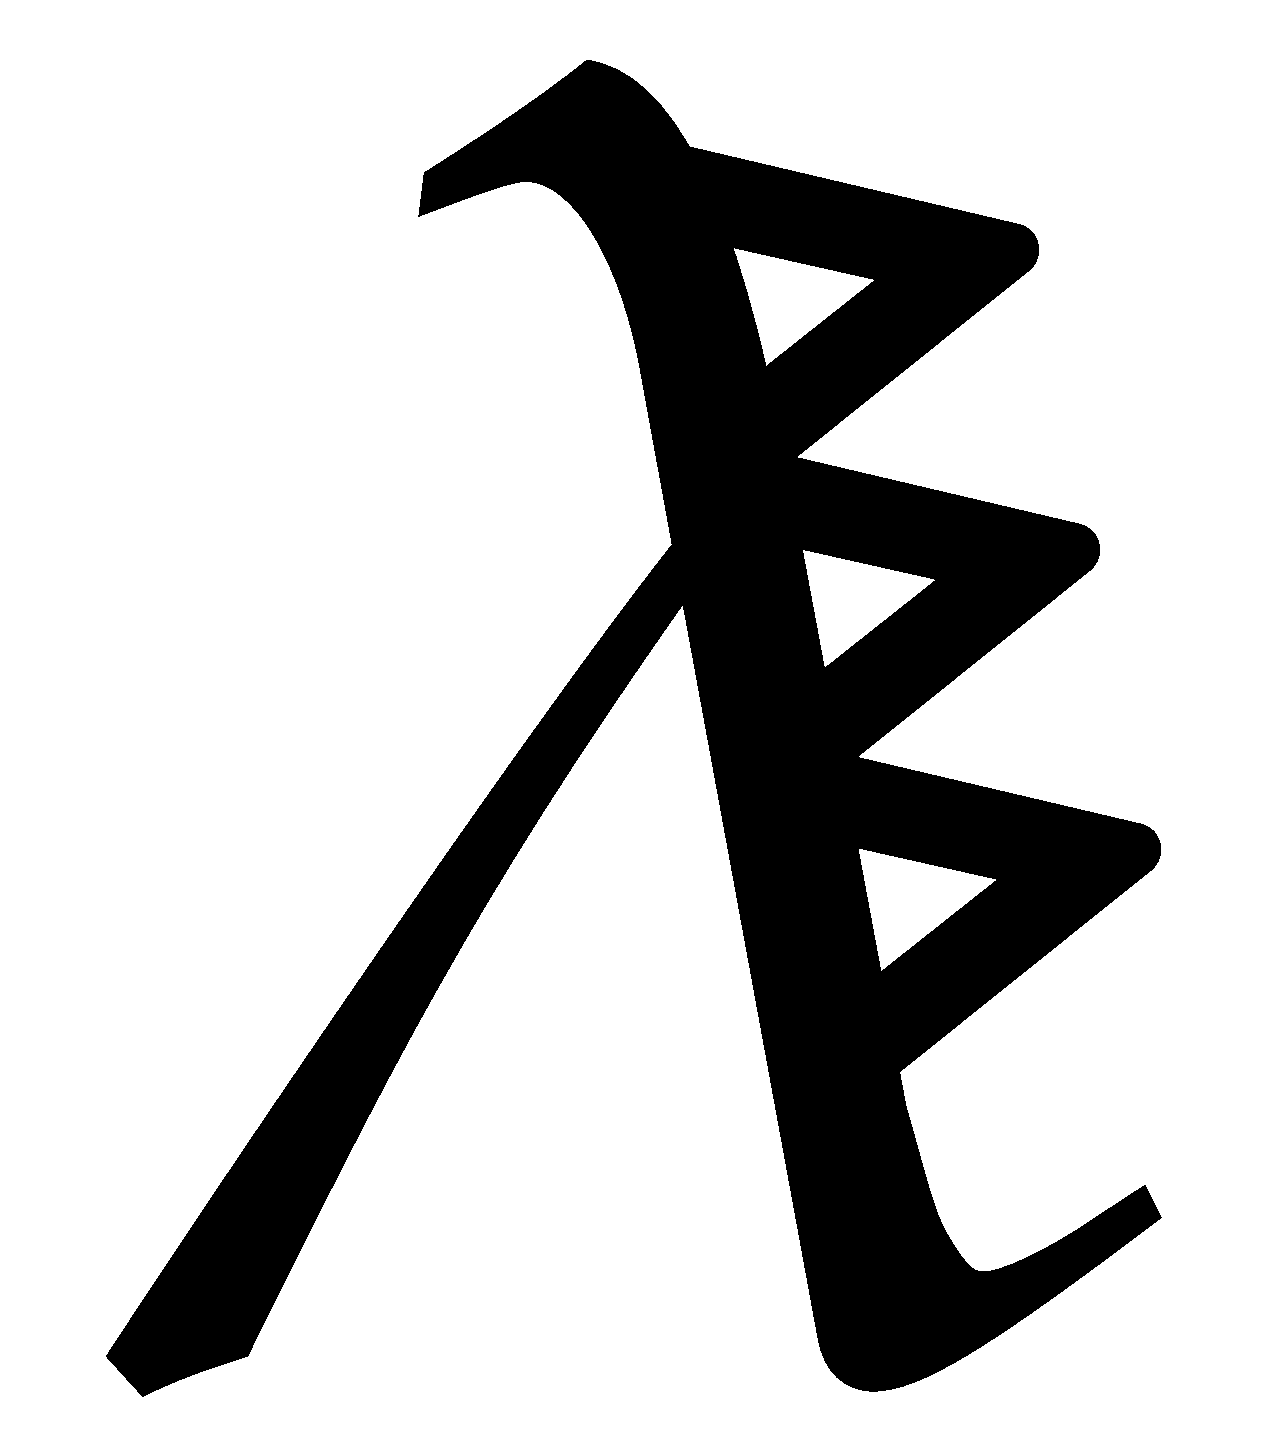
\includegraphics[scale=0.19]{spikyLambdaPazo.pdf}
			
			\vspace{5cm}
			\LARGE
				\textbf{Jinyan Miµ}\\
				Fall 2020\\
			\vspace{5cm}

		\vspace*{\fill}
		\end{center}			
	\end{titlepage}






	\LARGE \color{red}
		\noindent \textbf{Sets}\\
	\normalsize \color{black}
	
		\noindent A \textbf{Set} is a collection of objects which are called \textbf{Elements}.\\
		\note Let $S$ be a set, let $x$ is an element, then we have either $x \in S$ or $ x \notin S$.\\
		\note Order does not matter in a set. Repeats are not detected in a set.\\
		
		\noindent Let $X,Y$ be sets. $X$ is called a \textbf{Subset} of $Y$, denoted as $X \subseteq Y$, provided that every element of $X$ is an element of $Y$, that is, if, $X$ is a subset of $Y$, then for all $x \in X$, we have $x \in Y$. Moreover, if $X$ is a subset of $Y$, and $X \neq Y$, then we say $X$ is a \textbf{Proper Subset} of $Y$, denoted as $X \subset Y$.\\
	
		\noindent A set with no element in it is called an \textbf{Empty Set}, denoted as $\emptyset$.\\
		A set with exactly one element in it is called a \textbf{Singleton}.\\
		\note The empty set is a subset of every set.\\
	
		\noindent Let $a,b$ be elements. $(a,b) \coloneqq \{\{a\},\{a,b\}\}$ is called an \textbf{Ordered Pair}.\\
		\note By definition, we have $(a,b)=(c,d) \iff a=c \ and \ b=d$.\\
		
	
		\noindent Let $X$ be a set, let $A$ and $B$ be subsets of $X$:\\
		$A \cup B \coloneqq \{x \in X \mid x \in A \ or \ x \in B \}$  is called the \textbf{Union} of $A$ and $B$.\\
		$A \cap B \coloneqq \{x \in X \mid x \in A \ and \ x \in B \}$  is called the \textbf{Intersection} of $A$ and $B$.\\
		$A-B = A \setminus B \coloneqq \{x \in A \mid x \notin B \}$  is called the \textbf{Difference} between $A$ and $B$.\\	
		$X \setminus A \coloneqq \{x \in X \mid x \notin A \}$  is called the \textbf{Complement} of $A$ in $X$.\\
		$A \times B \coloneqq \{ (a,b) \mid a \in A \ and \ b \in B\}$ is called the \textbf{Cartesian Product} of the sets $A$ and $B$.\\
	
		\noindent Let $A,B$ be sets, let $f$ be a subset of $A \times B$. $f$ is called a \textbf{Function}, denoted as $f:A \to B \ \ \ x \mapsto f(x)$, provided that for all $a \in A$, there exists a unique $b \in B$ such that $(a,b) \in f$.\\
		\note The \textbf{Domain} of the function $f:A \to B$ is $A$, and the \textbf{Codomain} of $f$ is $B$.\\
	
		\noindent Let $X$ be a set. $\mathcal{P}(X) \coloneqq \{A \mid A \subseteq X\}$ is called the \textbf{Power Set} of $X$.\\
		\note The power set of a set $X$ is the set of all subsets of $X$.\\ 
	
		\noindent Let $S$ be a set. A function $\diamond : S \times S \to S$ is called a \textbf{Binary Operation} on $S$.\\
		\notation If $\diamond$ is a binary operation on a set $S$, for $s_1,s_2 \in S$, we write $s_1 \diamond s_2$ instead of $\diamond \, (s_1,s_2)$.\\
		\note If $\diamond$ is a binary operation on a set $S$, then $\diamond$ is a subset of $(S \times S) \times S$.\\
		\note Intersection and Union on a set $X$ are binary operations from $\mathcal{P}(X) \times \mathcal{P}(X)$ to $\mathcal{P}(X)$.\\
	
		\noindent Let $S$ be a set, let $f:S \to S$ and $g: S \to S$ be functions, let $Fun(S)\coloneqq \{h:S \to S\}$.\\ $\circ :Fun(S)\times Fun(S) \to Fun(S) \ \ \ (f,g)\mapsto f \circ g$ is a binary operation called \textbf{Function Composition}, and $(f \circ g): S \to S \ \ \ (f \circ g)(x)\mapsto f(g(x))$ is a function from $S$ to $S$ that sends $s \in S$ to $f(g(s))$.\\
	
		\noindent A binary operation $\diamond$ on a set $S$ is called \textbf{Commutative} provided that $\forall a,b \in S$, ${a \diamond b = b \diamond a}$.\\
	A binary operation $\diamond$ on a set $S$ is called \textbf{Associative} provided that $\forall a,b,c \in S$, ${(a \diamond b) \diamond c=a \diamond (b \diamond c)}$.\\
	
		\noindent Let $\diamond$ be a binary operation on $S$, the element $e \in S$ is called an \textbf{Identity} for $\diamond$ on $S$, denoted as $\diamond$-identity, provided that for all $s \in S$ we have $e \diamond s=s \diamond e = s$.\\
		\note The empty set can be an identity element of a binary operation on a set.\\
		\note 0 is not the identity of subtraction on $\R$.\\
	
		\noindent Let $S$ be a set, let $\diamond$ be a binary operation on $S$, let $e$ be a $\diamond$-identity. Given $s \in S$, an element $s' \in S$ is called an \textbf{Inverse} of $s$ with respect to $\diamond$ on $S$, denoted as $\diamond$-inverse, provided that $s \diamond s' = s' \diamond s = e$.\\
		
		\noindent Let $X$ be a set. The function $Id_X :X \to X \ \ \ x \mapsto x$ is called the \textbf{Identity Function} on X.\\

		\noindent Let $A$ and $B$ be sets, let $f:A \to B$ be a function. \\ $f$ is \textbf{Surjective} provided that $\forall b \in B, \ \exists \ a \in A \ s.t. \  f(a)=b$.\\ $f$ is \textbf{Injective} provided that $(f(a)=f(b)) \iff (a=b)$.\\ $f$ is \textbf{Bijective} provided that $f$ is both injective and surjective. \\
		\note Let $f$ be a bijection from set $A$ to set $B$, then $ \forall b \in B, \ \exists! \ a \in A, \ s.t. \ f(a)=b$.\\
	
		\noindent Let $A$ and $B$ be sets. a function $f:A \to B$ is said to be \textbf{Invertible} provided that $f^{-1}$ is a function. If $f$ is invertible, the function $f^{-1}:B \to A \ \ \ f^{-1}(b)=a \iff f(a)=b$ is called the \textbf{Inverse} of $f$.\\
		\note Given sets $A,B$ and $f:A \to B$, $f^{-1}=\{ (b,a) \in B \times A \mid (a,b) \in f \} $ is a subset of $B \times A$.\\
\clearpage
	
		\noindent Let $A$ and $B$ be sets, and let $f:A \to B$ be a function. The set $f(A) \coloneqq \{f(a)\in B \mid a \in A\}$ is called the \textbf{Image} of $f$.\\
		\note If $f(A)$ is the image of the function $f$ from set $A$ to set $B$, then $f(A)$ is a subset of $B$.\\
		
		\noindent Let $A,B$ be sets. The sets $A$ and $B$ are said to have the same \textbf{Cardinality} provided that exists a bijection from the set $A$ to the set $B$.\\

		\noindent Let $S$ be a set. A \textbf{Relation} on $S$ is a subset of $S \times S$.\\ Let $R$ be a relation on the set $S$, and let $x,y \in S$. We write $xRy$ whenever $(x,y) \in R$.\\

		\noindent Let $S$ be a set, let $R$ be a relation on $S$. $R$ is called an \textbf{Equivalence Relation} on $S$ provided that the followings hold:
		\begin{enumerate}[topsep=3pt,itemsep=-1ex,partopsep=1ex,parsep=1ex]
			\item $R$ is \textbf{Reflexive}, that is, $\forall s \in S$, we have $sRs$.
			\item $R$ is \textbf{Symmetric}, that is, $\forall s,t \in S$, if $sRt$, then $tRs$.
			\item $R$ is \textbf{Transitive}, that is, $\forall s,t,u \in S$, if $sRt$ and $tRu$, then $sRu$.
		\end{enumerate}
		If $R$ is an equivalence relation on $S$, then for $s,t \in S$, we write $s \sim t$ whenever $(s,t) \in R$.\\
		
		\noindent Let $S$ be a set, let $\sim$ be an equivalence relation on $S$, let $x \in S$. $C(x)\coloneqq \{ y \in S \mid y \sim x \}$ is called the \textbf{Class} of $x$ with respect to $\sim$, or the \textbf{Equivalence Class} of $x$ with respect to $\sim$.\\
		\notation If $C(x)$ is a class, then $C(x)$ can also be denoted as $[(x)]$.\\

		\noindent Let $S$ be a set, and let $\sim$ be an equivalence relation on $S$. The set $S/{\sim} \coloneqq \{ C(x) \mid x \in X\}$ is called the \textbf{Quotient} of $X$ with respect to $\sim$, or the \textbf{Factor Set} of $X$ with respect to $\sim$.\\
		
	\clearpage






	\LARGE \color{red}
		\noindent \textbf{Fields}\\
	\normalsize \color{black}
	
		\noindent Let $F$ be a set, let $\ast$ and $+$ be commutative and associative binary operations on $F$.\\ $(F,\ast,+)$ is called a \textbf{Field} provided that the followings hold:
		\begin{enumerate}[topsep=3pt,itemsep=-1ex,partopsep=1ex,parsep=1ex]
			\item There exists a $+$-identity in $F$, denoted as $0_F$.
			\item There exists a $\ast$-identity in $F$, denoted as $1_F$.
			\item For all $f \in F$, there exists a $+$-inverse of $f$ in $F$, denoted as $-f$.
			\item For all $f \in (F \setminus \{0_F\})$, there exists a $\ast$-inverse of $f$ in $F$, denoted as $f^{-1}$.		
			\item For all $a,b,c \in F$, we have $a \ast (b+c)=a\ast b+a\ast c$.
			\item $0_F \neq 1_F$.
		\end{enumerate}
		\note If $(F,\ast,+)$ is a field, then $F$ is not empty.\\
	
		\noindent A field $(F,+,\ast)$ is said to have an \textbf{Order Structure} provided that there exists a subset $P$ of the set $F$ such that the followings hold:
		\begin{enumerate}[topsep=3pt,itemsep=-1ex,partopsep=1ex,parsep=1ex]
			\item $P$ is closed with respect to the binary operations $+$ and $\ast$.
			\item For $a \in F$, \textbf{Trichotomy} holds: \ \ \ \
			\begin{inparaitem}
				\item $a \in P \ \ \ \ $    
				\item $-a \in P \ \ \ \ $    
				\item $a=0$
			\end{inparaitem}
		\end{enumerate}
		If $P$ satisfies the requirements listed above, then we say the pair $(F,P)$ has an ordered structure.
	
		\hfill\break
		\noindent A field $(F,+,\ast)$ is said to be \textbf{Ordered} provided that there exists a subset $P$ of $F$ such that $(F,P)$ has an ordered structure, and we called the pair $(F,P)$ an \textbf{Ordered Field}.\\
		\note Given $(F,P)$ is an ordered field, $P$ is always not empty.\\
		\note In general, a field can have more than one ordered structure.\\
	
		\noindent Let $(F,P)$ be an ordered field, let $a,b \in F$.\\
		We say $a$ is \textbf{Greater than} $b$, denoted as $a>b$, iff $(a-b)\in P$.\\
		We say $a$ is \textbf{Less than} $b$, denoted as $a<b$, iff $-(a-b)\in P$.\\
		We say $a$ is \textbf{Greater than or Equal to} $b$, denoted as $a \geq b$, iff $(a-b)\in P \cup \{0_F\}$.\\
		We say $a$ is \textbf{Less than or Equal to} $b$, denoted as $a \leq b$, iff $-(a-b)\in P \cup \{0_F\}$.\\
	
		\noindent Let $(F,P)$ be an ordered field.
		\\The function $| \ |: F \to F \ \ \ x \mapsto \begin{cases} x & x \in P \\ -x & -x \in P \\ 0_F & x=0_F \end{cases}$ is called the \textbf{Absolute Value Function} on $F$\\ 
		\hfill\break
		\hfill\break
		\noindent Let $(F,P)$ be an ordered field, let $a \in F$,  $|a|$ is called the \textbf{Absolute Value} of $a$.\\
		
		

		\hfill\break
		\hfill\break
		\noindent \color{red} Consider using the ordered field $(F,P)$ from now on. \color{black} \\
	
		\noindent Let $A$ be a subset of $F$, and let $u$ be an element in $F$. $u$ is called an \textbf{Upper Bound} for $A$ provided that for all $a \in A$, we have $u \geq a$. If $u$ is an upper bound for the set $A$, then we say the set $A$ is \textbf{Bounded Above} by $u$, and $A$ is bounded above in $F$.\\
	
		\noindent Let $A$ be a bounded above subset of $F$, and let $\alpha$ be an element in $F$. $\alpha$ is called a \textbf{Least Upper Bound} or \textbf{Supremum} for the set $A$ provided that the followings hold:
		\begin{enumerate}[topsep=3pt,itemsep=-1ex,partopsep=1ex,parsep=1ex]
			\item $\alpha$ is an upper bound for $A$.
			\item $\alpha$ is the least such, that is, if $u \in F$ is an upper bound for $A$, then $\alpha \leq u$.
		\end{enumerate}
		\note Not every set has a least upper bound.\\
		\note Empty set does not have a least upper bound.\\
		\note If a least upper bound exists for $A \subseteq F$, then it is unique.\\
		
		\noindent An ordered field $(F,P)$ is said to have the \textbf{Least Upper Bound Property} provided that every nonempty bounded above subset $A$ of $F$ has a least upper bound.\\
		
		\noindent An ordered field is said to be \textbf{Complete} provided that it has the least upper bound property.\\
		\note There exists a unique complete ordered field, called $\R$.\\
		
		\noindent Let $A$ be a subset of $F$, and let $w$ be an element in $F$. $w$ is called a \textbf{Lower Bound} for $A$ provided that for all $a \in A$, we have $w \leq a$. If $w$ is a lower bound for the set $A$, then we say the set $A$ is \textbf{Bounded Below} by $w$, and $A$ is bounded below in $F$.\\
		
		\noindent Let $A$ be a bounded below subset of $F$, and let $\beta$ be an element in $F$. $\beta$ is called a \textbf{Greatest Lower Bound} or \textbf{Infimum} for the set $A$ provided that the followings hold:
		\begin{enumerate}[topsep=3pt,itemsep=-1ex,partopsep=1ex,parsep=1ex]
			\item $\beta$ is a lower bound for $A$.
			\item $\beta$ is the greatest such, that is, if $w \in F$ is a lower bound for $A$, then $\beta \geq w$.
		\end{enumerate}
		\note Not every set has a greatest lower bound.\\
		\note Empty set does not have a greatest lower bound.\\
		\note If a greatest lower bound exists for $A \subseteq F$, then it is unique.\\
		
		\noindent Let $X$ be a subset of $F$, $X$ is said to be \textbf{Inductive} provided that the followings hold:\\
		\begin{inparaitem}
			\item $1_F \in X \ \ \ \ \ \ \ \ \ \ \ \ \ \ \ \ \ \ \ $
			\item If $x \in X$, then $x+1_F \in X$.
		\end{inparaitem}
	
		\hfill\break
		\noindent ${\N}_F \coloneqq \{ n \in F \mid n$ belongs to every inductive subset of $F \}$\\
		\noindent ${\Z}_F \coloneqq \{ z \in F \mid |z| \in {\N}_F \cup \{0\}\}$\\
		\noindent ${\Q}_F \coloneqq \{ q \in F \mid \exists \ z \in {\Z}_F$ and $n \in {\N}_F \ s.t. \  q=z \ast n^{-1} \} $\\
		\note When $F = \R$, then we have ${\N}_F=\N , \ {\Z}_F=\Z , \ {\Q}_F=\Q $.\\
		\note $\N$ is called the set of Natural Numbers, and $\Z$ is called the set of Integers.\\
		\note Rigorously, we define $\Q \coloneqq (\Z \times \N)/{\sim_{\Q}}$ with $(n_1,m_1)\sim_\Q (n_2,m_2) \iff (n_1 \cdot m_2 = n_2 \cdot m_1)$.\\
		\note $\Q$ is called the set of Rational Numbers.\\
	
		\noindent Let $B$ be a subset of $F$. $B$ is said to be  \textbf{Bounded} in $F$ provided that the set $B$ is both bounded above and bounded below in $F$.\\
		\fact Every nonempty bounded above subset of $R$ has a Supremum in $\R$.\\
		\fact Every nonempty bounded below subset of $R$ has a Infimum in $\R$.\\
		
		\noindent Let $A$ be a subset of $F$, let $m$ be an element in $F$. The element $m$ is called a \textbf{Maximal Element} for the set $A$ provided that $m$ belongs to $A$ and $m$ is an upper bound for $A$.\\
		
		\noindent Let $A$ be a subset of $F$, let $u$ be an element in $F$. The element $u$ is called a \textbf{Minimal Element} for the set $A$ provided that $u$ belongs to $A$ and $u$ is a lower bound for $A$.\\

		\noindent Let $A$ be a subset of $F$, let $b$ be an element in $F$.\\
		$-A \coloneqq \{-x \mid x \in A\} $\\
		$b+A \coloneqq \{b+x \mid x \in A\} $\\
		
		\noindent Let $U$ be a subset of $F$. $U$ is said to be \textbf{Well-ordered} provided that every nonempty subset of $U$ has a minimal element.\\
		
		\noindent Let $S$ be a subset of $\N$. $S$ is said to be \textbf{Weakly Inductive} provided that the followings hold:\\
		\begin{inparaitem}
			\item $1 \in S \ \ \ \ \ \ \ \ \ \ \ \ \ \ \ \ \ \ $
			\item If $k \in S$, then $(k+1) \in S$.\\
		\end{inparaitem}
		
		\noindent Let $S$ be a subset of $\N$. $S$ is said to be \textbf{Strongly Inductive} provided that the following holds:\\
		For all $n \in \N$, if the set $\{k \in \N \mid k< n \}$ is a subset of $S$, then $n$ is an element in $S$.\\
		
		\noindent Let $d,b \in \N$. the element $d$ is called a \textbf{Divisor} of $b$ provided that there exists $ m \in \N \ s.t. \ b=d \ast m$. 
		\notation If $d \in \N$ is a divisor of $b \in \N$, then we write $d\mid b$.\\
		
		\noindent Let $a,b \in \N$. The element $\gcd(a,b) \in \N$ is called the common divisor of $a$ and $b$ provided that $\gcd(a,b)$ is a divisor of both $a$ and $b$, and $\gcd(a,b)$ is the greatest such, that is, $\forall d \in \N$, if $d$ is a divisor of both $a$ and $b$, then we have $\gcd(a,b) \geq d$.\\
		
		\noindent The set $E \coloneqq \{ 2 \cdot k \mid k \in \Z \}$ is called the set of \textbf{Even Numbers} in $\R$.\\ The set $O \coloneqq \{ 2 \cdot k+1 \mid k \in \Z \}$ is called the set of \textbf{Odd Numbers} in $\R$.\\ Each element in $E$ is called an \textbf{Even Number}, and each element in $O$ is called an \textbf{Odd Number}.\\
		
		\noindent Let $S$ be a set, $S$ is said to be \textbf{Finite} provided that either $S$ is an empty set, or there exists a bijection from the set $N_n = \{ k \in \N \mid k<n \}$ to the set $S$ for some $n \in \N$. If there exists a bijection from $N_n$ to $S$ for some $n \in \N$, then we say $S$ has $n$ element.\\
		\note Let $S$ be a set, If there exists a bijection from $N_n$ to $S$ for some $n \in \N$, then $n$ is unique.\\
		
		\noindent Let $S$ be a set. $S$ is said to be \textbf{Infinite} provided that $S$ is not finite.\\		
		
		\noindent Let $S$ be a set. $S$ is \textbf{Countably Infinite} provided that there exists a bijection from $\N$ to $S$.\\
		
		\noindent Let $S$ be a set. $S$ is is said to be \textbf{Countable} provided that $S$ is either finite or countably infinite.\\
		\fact The sets $\N$, $\Z$, $\Q$ are all countable.\\
		\fact The sets $\R$ and $\R \setminus \Q$ are not countable.\\
		
		
		
		
		
		
		
		
		
		
		\noindent $i^2 \coloneqq -1$. The element $i$ is called the \textbf{Imaginary Unit}.\\
		
		\noindent Let $a,b \in \R$. $z \coloneqq a+bi$ is called a \textbf{Complex Number}, where $a$ is called the \textbf{Real Part} of $z$, $b$ is called the \textbf{Imaginary Part} of $z$, and $a+bi$ is called the \textbf{Cartesian Form} of $z$.\\ 
		
		\noindent $\Complex \coloneqq \{ a+bi \mid a,b \in \R \} $ is called the \textbf{Set of Complex Numbers}.\\
		\note The plane of complex numbers, called the \textbf{Complex Plane}, is a two dimensional plane.\\
		
		\noindent Let $z=a+bi,w=c+di$ be complex numbers, and let $k \in \R$.\\ $z+w \coloneqq (a+c)+(b+d)i$\\ $z \times w \coloneqq (a \times c - b \times d)+(a \times d + b \times c)i$\\ $z \times k \coloneqq (a \times k)+(b \times k)i$\\ $\bar{z} \coloneqq a-bi$ is called the \textbf{Conjugate} of $z$.\\ $|z| \coloneqq \sqrt{a^2+b^2}$ is called the \textbf{Absolute Value} or the \textbf{Modulus} of $z$.\\
		\fact Every nonzero complex number $z$ can be written as $z=|z|(cos(\theta)+i\sin(\theta))$ for some $\theta \in \R$.
		\note If $z$ is a complex number, then $\bar{z} \in \Complex$, $|z| \in \R$, $|z|$ is unique,\mbox{ and the absolute value of $\frac{z}{|z|}$ is $1$.}\\

		\noindent Let $z = a+bi = r(cos(\theta)+i\sin(\theta))=re^{i\theta}$ be a complex number. $\theta$ is called the \textbf{Argument} of $z$.\\ $r(cos(\theta)+i\sin(\theta))$ and $re^{i\theta}$ are called the \textbf{Polar Form} of $z$.\\
		\note If $z=re^{i\theta}$ is a complex number, then $r \in \R$ and $\theta \in \R$.\\
		\note If $z=re^{i\theta}$ is a complex number, then $r=|z|$ is unique, while $\theta$ is not unique.\\
		\fact Let $z \in \Complex$ and $z=re^{i\theta}$. If $\theta=\theta_0$ is one possibility, then the others are $\theta_0+2k \pi$ for $k \in \Z$.\\
		\fact If $z=re^{i\theta}=a+bi$ is a complex number, then $a=|z| \cos(\theta)$, $b=|z| \sin(\theta)$, $\theta = \tan^{-1}(\frac{b}{a})$.
		
	\clearpage





	
	\LARGE 	\color{red}
		\noindent \textbf{Topology}\\
	\normalsize	\color{black}
		
		\noindent Let $A$ be a subset of $\R$. $A$ is called an \textbf{Interval} provided that for all $x,y \in A$, if $z \in \R$ and $x<z<y$, then we have $z \in A$.\\
		
		\noindent Let $a,b \in \R$ with $a \leq b$. The followings are intervals:\\
		$(a,b) \coloneqq \{x \in \R \mid a<x<b \} \ \ \ \ \ \ \ \ \ \ \ \ \ \ \ \ \ \ \ \ \ \ \ \ \ \ \ \ [ \, a,b \, ] \coloneqq \{x \in \R \mid a\leq x\leq b \}$\\
		$\left( a,b \, ] \coloneqq \{x \in \R \mid a<x\leq b \} \ \ \ \ \ \ \ \ \ \ \ \ \ \ \ \ \ \ \ \ \ \ \ \ \ \ \ \ [ \, a,b \right) \coloneqq \{x \in \R \mid a\leq x<b \}$\\
		$\R_{>a}=(a,\infty) \coloneqq \{x \in \R \mid a<x \}  \ \ \ \ \ \ \ \ \ \ \ \ \ \ \ \ \ \ \ \ \ \ \ \R_{<b}=(-\infty,b) \coloneqq \{x \in \R \mid x< b \}$\\					$\R_{\geq a}=[\, a,\infty) \coloneqq \{x \in \R \mid a\leq x \}  \ \ \ \ \ \ \ \ \ \ \ \ \ \ \ \ \ \ \ \ \ \ \ \R_{\leq b}=(-\infty,b \, ] \coloneqq \{x \in \R \mid x\leq b \}$\\
		$(-\infty ,\infty )\coloneqq \{ x \in \R \}$\\
		
		\noindent Let $a,r \in \R$ with $r>0$. The set $B_r(a) \coloneqq \{ x \in \R \mid (a-r)<x<(a+r) \}$ is called the \textbf{Ball} centered at $a$ of radius $r$.\\

		\noindent $\T_{EUC} \coloneqq \{ A \subseteq \R \mid \forall a \in A,\ \exists \ r \in \R_{>0} \ s.t. \  B_r(a) \subseteq A\}$ is called the \textbf{Euclidean Topology} on $\R$.\\
		\note $\T_{EUC}$ is closed with respect to arbitrary unions and finite intersections.\\
		\note $\T_{EUC}$ is a set of sets, and $\T_{EUC}$ is a subset of $\mathcal{P} (\R )$.\\
		\note The pair $(\R, \T_{EUC})$ is a topological space.\\
		\note We have $\R \in \T_{EUC}$ and $\emptyset \in \T_{EUC}$.\\		
		
		\noindent Let $U$ be a subset of $\R$. The set $U$ is said to be \textbf{Open} in the Euclidean topology on $\R$ provided that $\forall u \in U,  \ \exists \ r \in \R_{>0}  \ s.t. \ B_r(u)\subseteq U$. Let $C$ be a subset of $\R$. The set $C$ is said to be \textbf{Closed} in the Euclidean topology on $\R$ provided that $\R \setminus C$ is open in the Euclidean topology on $\R$.\\
		\note Arbitrary union of open sets and finite intersection of open sets in $\T_{EUC}$ are open.\\
		\note The collection of all open subsets of $\R$ in the Euclidean Topology forms $\T_{EUC}$.\\
		\note Each element in $\T_{EUC}$ is called an open subset of $\R$.\\
		\note The empty set and $\R$ are both open and closed in $\T_{EUC}$.\\ 
		\note All balls are openin the Euclidean topology on $\R$. In  $(\R,\T_{EUC})$, balls are called \textbf{Open Balls}.\\



		\hfill\break
		\noindent \color{red} Consider using the topological space $(\R,\T_{EUC})$ from now on. \color{black} \\

		\noindent Let $p \in \R$. A \textbf{Neighborhood} of $p$ in $\T_{EUC}$ is an open interval in $\T_{EUC}$ that contains $p$.\\
		
		\noindent Let $f:\R \to \R$ be a function, let $a \in \R$. We say $f$ approaches $l$ as $x$ approaches $a$, denoted as $\lim_{x \to a} f = l$ for some $l \in \R$, provided that one of the followings holds:
		\begin{enumerate}[topsep=3pt,itemsep=-1ex,partopsep=1ex,parsep=1ex]
			\item For all $\epsilon >0, \ \exists \ \delta>0 \ s.t.$ if $x \in B_{\delta}(a) \setminus \{a \}$, then $f(x) \in B_{\epsilon}(l)$.
			\item For all $\epsilon >0, \ \exists \ \delta >0 \ s.t.$ if $x\in \R $ satisfies $0< |x-a| < \delta$, then $| f(x)-f(a) | < \epsilon$.
			\item For $V \in \T_{EUC}$, if $l \in V$, then $\exists \ U \in \T_{EUC} \ s.t \ a \in U$ and $\forall x \in U\setminus \{a \}$, we have $f(x) \in V$.
		\end{enumerate}
			\note The three statements are equivalent.\\
		\note $\lim_{x \to a} f$ is called the \textbf{Limit} of the function $f:\R \to \R$ at $a \in \R$.\\

		
		\noindent Let $f:\R \to \R$ be a function, let $a$ be an element in $\R$. The function $f$ is said to be \textbf{Continuous} at $a$ provided that one of the followings holds:
		\begin{enumerate}[topsep=3pt,itemsep=-1ex,partopsep=1ex,parsep=1ex]
			\item $\lim_{x \to a} f = l$ for some $l \in \R$ and $f(a)=l$.
			\item For all $\epsilon>0, \ \exists \ \delta>0 \ s.t.$ if $x \in B_{\delta}(a)$, then $f(x) \in B_{\epsilon}(f(a))$.
			\item For all $\epsilon >0, \ \exists \ \delta >0 \ s.t.$ if $x \in \R$ satisfies $| x-a | < \delta$, then $| f(x)-f(a) | < \epsilon$.
			\item For $V \in \T_{EUC}$, if $f(a) \in V$, then $\exists \ U \in \T_{EUC} \ s.t \ a \in U$ and $\forall x \in U$, we have $f(x) \in V$.
		\end{enumerate}
		\note The four statements are equivalent.\\
		
		\noindent Let $A,B$ be subsets of $\R$, let $f: A \to B$ be a function. $f$ is \textbf{Continuous} on $A$ provided that for all $a \in A,$ the function $f$ is continuous at $a$. If a function $f$ is continuous on its domain, then we say the function $f$ is \textbf{Continuous}.\\

		\noindent Let $A,B$ be subsets of $\R$, let $S$ be a subset of $A$, let $f:A \to B$ be a function.\\ The \textbf{Restriction} of $f$ to $S$ is the function from $S$ to $B$ that sends $s \in S$ to $f(s)$, such function is denoted as $res_S f:S \to B$. Moreover, the image of $res_S f$ is denoted as $f([S])$ or $f(S)$ or $res_S f(S)$.\\
		
		\noindent By Theorem, we can redefine the continuity of a function $f:\R \to \R$: The function $f:\R \to \R$ is said to be \textbf{Continuous} provided that for all $U \in \T_{EUC}$, we have $f^{-1}(U) \in \T_{EUC}$.\\
		
		\noindent \color{red} The assumption of using $(\R,\T_{EUC})$ is removed. \color{black}
	\clearpage

		\noindent  Let $X$ be a set. A \textbf{Topology} $\T_X$ on the set $X$ is a subset of $\Power (X)$ that satisfies the followings:
		\begin{enumerate}[topsep=3pt,itemsep=-1ex,partopsep=1ex,parsep=1ex]
			\item The set $X$ and the empty set are in $\T_X$.
			\item $\T_X$ is closed with respect to arbitrary union.
			\item $\T_X$ is closed with respect to finite intersection.
		\end{enumerate}
		\note A set can have more than one topology.\\
		
		\noindent Let $X$ be a set, let $\T_X$ be a topology on $X$. The pair $(X, \T_X)$ is called a \textbf{Topological Space}.\\
		
		\noindent Let $(X,\T_X)$ be a topological space. Each the element in $\T_X$ is called an \textbf{Open Subset} of $X$ in $\T_X$, that is, let $U$ be a subset of $X$, the set $U$ is said to be \textbf{Open} if and only if $U$ belongs to $\T_X$.\\
		
		\noindent Let $(X,\T_X)$ be a topological space, let $p \in X$. A \textbf{Neighborhood} of $p$ in $\T_X$ is an open set in $\T_X$ that contains $p$.\\
		
		\noindent Let $(X,\T_X)$ and $(Y,\T_Y)$ be topological spaces. The function $f:X \to Y$ is said to be \textbf{Continuous} provided that for all $u \in \T_Y$, we have $f^{-1}(u) \in \T_X$.\\
		
		\noindent Let $(X,\T_X)$ and $(Y,\T_Y)$ be topological spaces. The function $f:X \to Y$ is \textbf{Locally Constant} provided that $\forall x \in X$, $\exists$ a neighborhood $U$ of $x$ in $\T_X \ s.t. \ \forall y \in U$, we have $f(y)=c$ for some $c \in Y$.\\
		
		\noindent Let $(X,\T)$ be a topological space, let $A$ be a subset of $X$. The intersection of all closed subsets of $X$ that contain $A$ is called the \textbf{Topological Closure} of $A$ in $\T$, denoted as $\bar{A}$.\\
		
		\noindent Let $(X,\T)$ be a topological space, let $A$ be a subset of $X$. The union of all open sets that are contained in $A$ is called the \textbf{Interior} of $A$ in $\T$, denoted as $\texttt{int}(A)$.\\ 
		
		\noindent Let $X$ be a set. The \textbf{Indiscrete Topology} on $X$, denoted as $\T_{ind}$, contains only $\emptyset$ and $X$.\\ Let $X$ be a set. The \textbf{Discrete Topology} on $X$, denoted as $\T_{dis}$, contains all subsets of $X$.\\
		\note In the discrete topology on the set $X$, every subset of $X$ is both open and closed.\\
		\note Let $X$ be a set. $\T_{ind} =\{\emptyset, X\}$ and $\T_{dis} = \Power (X)$.\\
		
		\noindent Let $(X,\T_X)$ be a topological space. If $A$ is a subset of $X$, then $A$ inherits the structure of the topological space from $X$, that is, $\T_A \coloneqq \{ U \cap A \mid U \in \T_X \}$ is the \textbf{Subspace Topology} on $A$, each element in $\T_A$ is called an \textbf{Open Subset} of $A$ in the subspace topology of $A$.\\
		
		\noindent In $(\R,\T_{EUC})$, let $A$ be a subset of $\R$, let $\T_A$ denote the subspace topology on $A$, let $f:A \to \R$ be a function. let $a$ be an element in $A$. We say $f$ approaches $l$ as $x$ approaches $a$, denoted as $\lim_{x \to a} f = l$ for some $l \in \R$, provided that one of the followings holds:
		\begin{enumerate}[topsep=3pt,itemsep=-1ex,partopsep=1ex,parsep=1ex]
		\item For all $\epsilon >0, \ \exists \ \delta >0 \ s.t.$ if $x \in (B_{\delta}(a) \setminus \{ a \} )\cap A$, then $f(x) \in B_{\epsilon}(l)$.
		\item For all $\epsilon >0, \ \exists \ \delta >0, \ s.t.$ if $x \in A$ satisfies $|x-a|<\delta$, then $|f(x) - f(a)| < \epsilon$.
		\item For $V \in \T_{EUC}$, if $l \in V$, then $\exists \ U \in \T_A \ s.t. \ a \in U$ and $\forall x \in (U \setminus \{a \})\cap A$, we have $f(x) \in V$.
		\end{enumerate}
		\note The three statements are equivalent.\\
		\note Let $A$ be a subset of $\R$. $\lim_{x \to a} f$ is called the \textbf{Limit} of the function $f:A \to \R$ at $a \in A$.\\

		\noindent In $(\R,\T_{EUC})$, let $A$ be a subset of $\R$, let $\T_A$ denote the subspace topology on $A$, let $f:A \to \R$ be a function, let $a$ be an element in $A$, $f$ is \textbf{Continuous} at $a$ provided that one of the followings holds:
		\begin{enumerate}[topsep=3pt,itemsep=-1ex,partopsep=1ex,parsep=1ex]
			\item $\lim_{x \to a} f = l$ for some $l \in \R$ and $f(a)=l$.		
			\item For all $\epsilon>0, \ \exists \ \delta>0 \ s.t.$ if $x \in B_{\delta}(a) \cap A$, then $f(x) \in B_{\epsilon}(f(a))$.
			\item For all $\epsilon >0, \ \exists \ \delta >0 \ s.t.$ if $x \in A$ satisfies $| x-a | < \delta$, then $| f(x)-f(a) | < \epsilon$.
			\item For $V \in \T_{EUC}$, if $f(a) \in V$, then $\exists \ U \in \T_A \ s.t \ a \in U$ and $\forall x \in U \cap A$, we have $f(x) \in V$.
		\end{enumerate}
		\note The four statements are equivalent.\\
		\note By definition, if $f:A \to \R$ is continuous at $a \in A$, then  $f:A \to f(A)$ is continuous at $a$.\\
		\note By definitions, if the function $f:A \to \R$ is continuous, then  $f:A \to f(A)$ is continuous.\\
		
		\noindent A topological space $(X,\T_X)$ is said to be \textbf{Disconnected} provided that there exist nonempty disjoint subsets $A,B \in \T_X$ such that $A \cup B = X$. A topological space $(Y,\T_Y)$ is said to be \textbf{Connected} provided that $(Y,\T_Y)$ is not disconnected.\\
		\fact Let $X$ be a set. The topological space $(X,\T_{ind})$ is always connected.\\
		\fact In $(\R,\T_{EUC})$, let $A$ be a subset of $\R$, let $\T_A$ denote the subspace topology on $A$. The topological space $(A,\T_A)$ is connected if and only if $A$ is an interval.\\
		

\clearpage
		
				
		\noindent Let $(X,\T)$ be a topological space, let $A$ be a subset of $X$. A collection of open sets $\C \subseteq \T$ is called an \textbf{Open Cover} of $A$ in $\T$ provided that $A \subseteq \bigcup_{C \in \C} C$.\\
		
		\noindent Let $(X,\T)$ be a topological space, let $A$ be a subset of $X$, and let $\C$ be an open cover of $A$ in $\T$. A subcollection $\C '$ of $\C$ is called an \textbf{Open Subcover} of $A$ in $\T$ provided that $A \subseteq \bigcup_{C' \in \C'}C'$.\\
		
		\noindent Let $(X,\T)$ be a topological space, let $A$ be a subset of $X$, let $\T_A$ denote the subspace topology on $A$ inherited from $\T$. The topological space $(A,\T_A)$ is said to be \textbf{Compact} provided that every open cover of $A$ in $\T$ admits a finite open subcover in $\T$.\\
		\fact The topological space $(\R,\T_{EUC})$ is not compact.\\	
		\fact If $X$ is a finite set, then the topological space $(X,\T)$ is always compact.\\	
		\fact Let $a,b \in \R$ with $a<b$, let $(a,b)$ be an interval, let $\T_{(a,b)}$ denote the subspace topology on $(a,b)$. The topological space $((a,b),\T_{(a,b)})$ is not compact.\\
		
		\noindent Let $(X,\T)$ be a topological space, let $x,y \in X$. A \textbf{Path} connecting $x$ and $y$ is a continuous function $f:[\, 0,1 \, ] \to X$ such that $f(0)=x$ and $f(1)=y$.\\

		
		\noindent Let $(X,\T)$ be a topological space. The topological space $(X,\T)$ is said to be \textbf{Path Connected} provided that for all $x,y \in X$, there exists a path connecting $x$ and $y$.\\
		\note If the topological space $(X,\T)$ is path connected, then $(X,\T)$ is connected.\\
		\note The connectedness of a topological space does not imply its path connectedness.\\
		
		\noindent $\R^2 \coloneqq \R \times \R = \{ (x,y) \mid x,y \in \R \}$\\
		$\R^3 \coloneqq (\R \times \R) \times \R = \{ (x,y,z) \mid x,y,z \in \R \}$\\
		
		\noindent Let $X$ be a set. $d:X \times X \to \R_{\geq 0}$ is called a \textbf{Metric} on $X$ provided that the followings hold:
		\begin{enumerate}[topsep=3pt,itemsep=-1ex,partopsep=1ex,parsep=1ex]
			\item For all  $x,y \in X,$ we have $d(x,y)=d(y,x)$.
			\item For $x,y \in X$, $d(x,y)=0$ if and only if $x=y$.
			\item For all $x,y,z \in X$, we have $d(x,y)\leq (d(x,z)+d(z,y))$.
		\end{enumerate}
		
		\hfill\break
		\noindent The function $d_3: \R^3 \times \R^3 \to \R_{\geq 0} \ \ \ ((x_1,y_1,z_1),(x_2,y_2,z_2)) \mapsto \sqrt{(x_1-x_2)^2+(y_1-y_2)^2+(z_1-z_2)^2}$ is called the Euclidean metric, or Euclidean distance, on $\R^3$.\\ The function $d_2: \R^2 \times \R^2 \to \R_{\geq 0} \ \ \ ((x_1,y_1),(x_2,y_2)) \mapsto \sqrt{(x_1-x_2)^2+(y_1-y_2)^2}$ is called the Euclidean metric, or Euclidean distance, on $\R^2$.\\ The function $d_1:\R \times \R \to \R_{\geq 0} \ \ \ x \mapsto \mid x \mid$ is called the Euclidean metric, or Euclidean distance, on $\R$.\\
				
		\noindent Let $X$ be a set, let $d_X$ be a metric on $X$. The pair $(X,d_X)$ is called a \textbf{Metric Space}.\\				

		\noindent Let $(X,d)$ be a metric space, let $a \in X$, and let $r>0$. The set $B_r \coloneqq \{ x \in X \mid d(x,a)<r \} $ is called a \textbf{Ball} centered at $a$ of radius $r$.\\ 
		
		\noindent Let $(X,d)$ be a metric space. $\T_d \coloneqq \{ A \subseteq X \mid \forall a \in A, \ \exists \ r>0 \ s.t. \ B_r(a) \subseteq A \}$ is the \textbf{Topology on $X$ associated to $d$}. In the topological space $(X,\T_d)$, let $A$ be a subset of $X$. The set $A$ is said to be \textbf{Open} in $\T_d$ provided that for all $a \in A$, there exists $r>0$ such that $B_r(a)$ is a subset of $A$.\\
		
		\noindent A topological space $(X,\T)$ is said to be \textbf{Metrizable} provided that $\exists$ a metric $d$ on $X \ s.t \ \T_d = \T$.\\
		\note Let $(X,d)$ be a metric space, and let $a \in X$, then $B_r(a) \in \T_d$.\\
		\note Indiscrete topology is not metrizable.\\
		\note Discrete topology is metrizable.\\

		
		\noindent Let $d_1,d_2,d_3$ denote the Euclidean metric on $\R,\R^2,\R^3$, respectively, and let $r \in \R$.\\ $S^0 \coloneqq \{ x \in \R \mid d_1(x,0)=r \}$ is a zero-dimensional sphere of radius $r$ in $\R$.\\ $S^1 \coloneqq \{ (x,y) \in \R^2 \mid d_2((x,y),(0,0))=r \}$ is an one-dimensional sphere of radius $r$ in $\R^2$.\\ $S^2 \coloneqq \{ (x,y,z) \in \R^3 \mid d_2((x,y,z),(0,0,0))=r \}$ is a two-dimensional sphere of radius $r$ in $\R^3$.\\
		\note A zero-dimensional sphere is often called an open ball in $\R$.\\
		\note A one-dimensional sphere is often called a circle in $\R^2$.\\
		\note A two-dimensional sphere is often called a sphere in $\R^3$.\\
		
		\noindent Let $(X,\T_X)$ and $(Y,\T_Y)$ be topological spaces, let $f:X \to Y$ be a function. $f$ is called an \textbf{Open Map} from $(X,\T_X)$ to $(Y,\T_Y)$ provided that for all $V \in \T_X$, we have $f(V) \in \T_Y$.\\
\clearpage

		\noindent Let $(X,\T_X)$ and $(Y,\T_Y)$ be topological spaces, let $f:X \to Y$ be a function. The function $f$ is called a \textbf{Homeomorphism} from $(X,\T_X)$ to $(Y,T_Y)$ provided that the followings hold:
		\begin{enumerate}[topsep=3pt,itemsep=-1ex,partopsep=1ex,parsep=1ex]
			\item $f:X \to Y$ is bijective.
			\item $f:X \to Y$ is continuous.
			\item $f^{-1}:Y \ to X$ is continuous.
		\end{enumerate}
		\fact Let $(X,\T_X)$ and $(Y,\T_Y)$ be topological spaces. If $f:X \to Y$ is a homeomorphism from $(X,\T_X)$ to $(Y,\T_Y)$, then the inverse of $f$, $f^{-1}:Y \to X$ is a homeomorphism from \mbox{$(Y,\T_Y)$ to $(X,\T_X)$}.\\
		\fact Let $(X,\T_X)$ and $(Y,\T_Y)$ be homeomorphic topological spaces, let $h:X \to Y$ be a homeomorphism, let $A$ be a subset of $X$, let $\T_A$ and $\T_{h(A)}$ be subspace topology, the restriction of $h$ on $A$, $res_A h:A \to h(A)$, is a homeomorphism from $(A,\T_A)$ to $(h(A), \T_{h(A)})$.\\
		
		\noindent Let $(X,\T_X)$ and $(Y,\T_Y)$ be topological spaces. The topological space $(X,\T_X)$ is said to be \textbf{Homeomorphic} to $(Y,\T_Y)$ provided that there exists a homeomorphism from $(X,\T_X)$ to $(Y,\T_Y)$.\\
		\note Being homeomorphic defines an equivalence relation on topological spaces.\\
		\fact Let $\T_{EUC_2}$ denote the topology on $\R^2$ associated to the Euclidean metric on $\R^2$. The topological space $(\R^2, \T_{EUC_2})$ is not homeomorphic to the topological space $(\R, \T_{EUC})$.\\	
 	
		
		\noindent Let $(X,\T)$ be a connected topological space, let $x \in X$, let $\T_{x}$ denote the subspace topology on the set $X \setminus \{x\}$ inherited from $\T$. $x$ is called a \textbf{Cut Point} of $X$ provided that $(X \setminus \{x\}, \T_x)$ is disconnected, and $cut(X) \coloneqq \{ x \in X \mid x$ is a cut point of $X \} $ denotes the set of cut point of $X$.\\
		\fact Let $(X,\T_X)$ and $(Y,\T_Y)$ be connected homeomorphic topological spaces, any homeomorphism between $(X,\T_X)$ and $(Y,\T_Y)$ sends cut point to cut point, that is, if $h:X \to Y$ is a homeomorphism from $(X,\T_X)$ to $(Y,\T_Y)$, then the restriction of $h$ on $cut(X)$, $res_{cut(X)}h:cut(X) \to cut(Y)$, is a bijection from $cut(X)$ to $cut(Y)$.\\
		
		\noindent Let $(X,\T_X)$ be a topological space. $(X,\T_X)$ is said to be \textbf{Totally Disconnected} provided that the only connected subsets of $X$ are the singletons and the empty set.\\
		\note $(\R,\T_{dis}),\ (\Z,\T_{EUC}),\ (\N,\T_{EUC}),\ (\Q,\T_{EUC}),\ (\R \setminus \Q,\T_{EUC})$ are totally disconnected.\\
		
		\noindent Let $(X,\T_X)$ be a topological space, let $A$ be a subset of $X$. The element $a \in A$ is called an \textbf{Isolated Point} of $A$ provided that $\exists \ U \in \T_X \ s.t. \ a \in U$ and $U \cap (A \setminus \{a\})= \emptyset$, that is, there exists an open subset $U$ of $X$ such that $U$ contains $a$ and $U$ contains no other elements of $A$.\\ 
		\note In $(\R,\T_{EUC})$, all elements in $\N$ are isolated points of $\N$.\\
		\note In $(\R,\T_{EUC})$, all elements in $\Z$ are isolated points of $\Z$.\\
		\note In $(\R,\T_{EUC})$, $\Q$ has no isolated point.\\
		\fact Let $(X,\T_X)$ be a topological space, let $A$ be a subset of $X$. If $a \in A$ is an isolated point of $A$, then $\{a\}$ is open in the subspace topology on the set $A$ inherited from $\T_X$.\\	

		\noindent Let $(X,\T_X)$ be a topological space, let $A$ be a subset of $X$. The set $A$ is said to be \textbf{Perfect} provided that $A$ is closed in $\T_X$ and $A$ has no isolated point.\\
		
		\noindent Let $(X,\T_X)$ be a topological space, let $A$ be a subset of $X$. The element $a \in X$ is called a \textbf{Limit Point} of $A$, or an \textbf{Accumulation Point} of $A$, provided that $\forall \ U \in \T_X$, if $a \in U$, then $\exists \ a' \in A \setminus \{a\} \ s.t. \ a' \in U$, that is, for all open subsets $U$ of $X$ that contain $a$, we have $U \cap (A \setminus \{a\}) \neq \emptyset$.\\
		\note In $(\R,\T_{EIC})$ any singleton subset of $\R$ has no accumulation point.\\
		
		\noindent Let $(X,\T_X)$ be a topological space. The topological space $(X,\T_X)$ is said to be \textbf{Hausdorff} provided that for all distinct $x,y \in X$, there exist disjoint $U,V \in \T_X \ s.t. \ x \in U$ and $y \in V$.\\
		\note In a Hausdorff space, we can separate distinct points with open sets.\\		
		
		\noindent Let $(X,d_X)$ and $(Y,d_Y)$ be metric spaces, let $f:X \to Y$ be a function. $f$ is said to be \textbf{Lipschitzian} provided that there exists $c \in \R$ such that $\forall x,y \in X$, we have $d_Y(f(x),f(y)) \leq c \cdot d_X(x,y)$.\\
		
		\noindent \textbf{Topological Invariants} are the properties of  topological spaces that are preserved by homeomorphisms between topological spaces.
		
	\clearpage






	\LARGE \color{red}
		\noindent \textbf{Groups}\\
	\normalsize \color{black}	
	
		\noindent A set $G$ with a binary operation $\diamond$ on $G$ is called a \textbf{Group} provided that the followings hold:
		\begin{enumerate}[topsep=3pt,itemsep=-1ex,partopsep=1ex,parsep=1ex]
			\item The binary operation $\diamond$ is associative.
			\item There exists $\diamond$-identity $e \in G$.
			\item For all $g \in G$, there exists $h \in G$ such that $g \diamond h =h \diamond g =e$.
		\end{enumerate}
		\note If $(G,\diamond)$ is a group, then the $\diamond$-inverse of each $g \in G$ is unique.\\
		\note The followings are groups: $(\R,+)$,\ \ \ $(\Z,+)$,\ \ \ $(\R \setminus \{0 \},\ast)$,\ \ \ $((0,\infty),\ast)$\\
		\note The followings are not group: $(\R,\ast)$,\ \ \ $(\N, +)$, \ \ \ $([\,0,\infty),\ast)$\\
		\note Let $(F,+,\ast)$ be a filed, $(F,+)$ and $(F\setminus \{0_F\}, \ast)$ are groups.\\
		
		\noindent Let $(G,\diamond_G),(H,\diamond_H)$ be groups, let $\varphi :G \to H$ be a function, $\varphi$ is called a \textbf{Group Homomorphism} from $(G,\diamond_G)$ to $(H,\diamond_H)$ provided that for $a,b \in G$, we have $\varphi \, (a \diamond_G b) = \varphi\, (a) \diamond_H \varphi\, (b)$.\\
		\fact Let $(G,\diamond_G),(H,\diamond_H)$ be groups. The function  $\varphi :G \to H$ that sends all elements in $G$ to the $\diamond_H$-identity in $H$ is a group homomorphism from $(G,\diamond_G)$ to $(H,\diamond_H)$.\\
		
		\noindent Let $(G,\diamond_G),(H,\diamond_H)$ be groups, let $\varphi :G \to H$ be a group homomorphism from $(G,\diamond_G)$ to $(H,\diamond_H)$. $\varphi$ is called a \textbf{Group Isomorphism} from $(G,\diamond_G)$ to $(H,\diamond_H)$ provided that $\varphi$ is a bijection from $G$ to $H$. If $\varphi$ is a group isomorphism from $(G,\diamond_G)$ to $(H,\diamond_H)$, then $(G,\diamond_G)$ is Isomorphic to $(H,\diamond_H)$.\\
		\fact Let $(G,\diamond_G),(H,\diamond_H)$ be groups. If $\varphi :G \to H$ is a group isomorphism from $(G,\diamond_G)$ to $(H,\diamond_H)$, then the inverse of $\varphi$, $\varphi^{-1} :H \to G$, is a group isomorphism from $(H,\diamond_H)$ to $(G,\diamond_G)$.\\
		\fact The group $((0,\infty),\ast)$ is isomorphic to the group $(\R,+)$.\\
		
		\noindent Let $(G,\diamond_G),(H,\diamond_H)$ be groups, let $e_H \in H$ be the $\diamond_H$-identity, let $\varphi :G \to H$ be a group homomorphism from $(G,\diamond_G)$ to $(H,\diamond_H)$. $im(\varphi) \coloneqq \{ \varphi(g) \mid g \in G\}$ is called the \textbf{Image} of $\varphi$. $ker(\varphi) \coloneqq \{ g \in G \mid \varphi(g)=e_H \}$ is called the \textbf{Kernel} of $\varphi$.\\
		
		\noindent A group $(G,\diamond)$ is said to be \textbf{Abelian} provided that $\diamond$ is commutative.\\
		
		\noindent Let $n \in \N$, let $X_n=\{x_1,x_2,x_3,\cdots,x_n\}$ be a finite set. A bijection $f:X_n \to X_n$ is called a \textbf{Permutation} of the set $X_n$, and the set $s_n \coloneqq \{ f: X_n \to X_n \mid f$ is bijective$\}$ is called the \textbf{Collection of the Permutations} of the finite set $X_n$.\\
 		\note Let $n \in \N$, let $\circ$ denote function composition. $S_n \coloneqq (s_n, \circ)$ is a group.\\
		\fact Let $n \in \N$, the set $s_n$ has $n!$ element.\\

		 
		\noindent Let $n \in \N$, $S_n \coloneqq (s_n, \circ)$ is called the \textbf{Symmetric Group on $n$ Letters}.\\
		\fact For $n \in \N$ with $n \geq 3$, the group $S_n$ is not abelian.\\
		
		\noindent Let $n \in \N$ with $n\geq 3$, given a regular polygon with $n$ sides. a \textbf{Dihedral Group}, denoted as $D_n$ is the group of symmetries of the n-sided regular polygon, which includes rotations and reflections of the n-sided regular polygon.\\
		\fact Let $n \in \N$ with $n\geq 3$, the group $D_n$ has $2n$ elements.\\
		\fact Let $n \in \N$ with $n\geq 3$, the group $D_n$ is not abelian.\\
		\fact Let $n \in \N$ with $n >3$, $D_n$ is not isomorphic to $S_n$.\\		
		
	\clearpage
		
		
		
		
		
		
		
		
		
		
		
		
		
		
		
		
		
		
		
		
		
		
		
		


		
		
		
		
		
			

	\color{red}
	\LARGE
		\noindent \textbf{Calculus}\\
	
	\normalsize
	\color{black}	
	
		\noindent \color{red} Consider using the topological space $(\R, \T_{EUC})$ from now on.\\ Fix $a,b \in \R$ with $a<b$, $n \in \N$, consider using the interval $[\,a,b\,]$  from now on. \color{black} \\
		
		\noindent Let $M,B$ be a subset of $\R$, let $A$ be a subset of $M$, let $f:M \to B$ be a function.\\ $f$ is \textbf{Strictly Increasing} on $A$ provided that if $x,y \in A$ with $x<y$, then $f(x)<f(y)$.\\ $f$ is \textbf{Strictly Decreasing} on $A$ provided that if $x,y \in A$ with $x<y$, then $f(x)>f(y)$.\\ $f$ is \textbf{Non-Decreasing} on $A$ provided that if $x,y \in A$ with $x<y$, then $f(x)\leq f(y)$.\\ $f$ is \textbf{Non-Increasing} on $A$ provided that if $x,y \in A$ with $x<y$, then $f(x)\geq f(y)$.\\  $f$ is called a \textbf{Constant Function} on $A$ provided that $\exists \ k \in \R \ s.t. \ \forall c \in f(A), \ c=k$.\\ $f$ is \textbf{Bounded} on $A$ provided that the set $f(A)$ is bounded.\\ $f$ is \textbf{Non-Negative} on $A$ provided that $\forall c \in f(A), \ c\geq 0$.\\ $f$ is \textbf{Non-Positive} on $A$ provided that $\forall c \in f(A), \ c\leq 0$.\\ $f$ is \textbf{Negative} on $A$ provided that $\forall c \in f(A), \ c < 0$.\\$f$ is \textbf{Positive} on $A$ provided that $\forall c \in f(A), \ c> 0$.\\
		\fact Let $A,B$ be subsets of $\R$, let $f:A \to B$ be a function. If $f$ is bounded on $A$, then there exists $m \in \R$ such that for all $x \in A$, we have $|f(x)| \leq m$.\\
		
		\noindent Let $A,B$ be subsets of $\R$, let $f:A \to B$ be a function. $f$ is said to be \textbf{Locally Bounded} on $A$ provided that for all $x \in A$, there exists a neighborhood $U$ of $x$ such that $f$ is bounded on $U$.\\ 
		
		\noindent Let $A,B$ be subsets of $\R$, let $f:A \to B$ be a function. $f$ is said to be \textbf{Locally Constant} on $A$ provided that for all $x \in A$, $ \exists \ \epsilon >0$ such that for all $y \in B_\epsilon(x)$, we have $f(y) =d $ for some $d \in \R$.\\		
		
		\noindent Let $A,B$ be subsets of $\R$, let $f:A \to B$ be a function. $f$ is said to be \textbf{Uniformly Continuous} on $A$ provided that $\forall \epsilon>0, \ \exists \ \delta>0 \ s.t.$ if $x,y \in A$ with $|x-y|<\delta$, then $|f(x)-f(y)|<\epsilon$.\\
		\fact Let $A \subseteq \R$. If $f:A \to \R$ is uniformly continuous on $A$, then $f$ is continuous on $A$.\\

		\noindent Let $a,b \in \R$, let $[\,a,b\,]$ be an interval, $l\coloneqq b-a$ is called the \textbf{Length} of $[\,a,b\,]$.\\
		
		\noindent An ordered set $P \coloneqq \{ t_0,t_1,t_2,\cdots ,t_n \}$ of points in $\R$, where $a=t_0<t_1<t_2<\cdots<t_n=b$, is called a \textbf{Partition} of $[\,a,b\,]$. For $i \in \N, \ 1\leq i \leq n$, the interval $[t_{i-1},t_i]$ is called a \textbf{Subinterval} of $P$. \\
		
		
		\noindent Let $P = \{ t_0,t_1,t_2,\cdots ,t_n \}$ be a partition of $[\,a,b\,]$. If the length of each subinterval of $P$ is $\frac{b-a}{n}$, that is, for $i \in \N, \ 0\leq i \leq n, \ t_i=a+\frac{b-a}{n}i$, then $P$ is called a \textbf{Regular Partition} on $[\,a,b\,]$.\\		
		
		\noindent Let $P,Q$ be partitions of $[\,a,b\,]$, $Q$ is called a \textbf{Refinement} of $P$ provided that $P$ as a set is a subset of the set $Q$, and we write $P \leq Q$ if $Q$ is a refinement of $P$.\\

		\noindent Let $P = \{ t_0,t_1,t_2,\cdots ,t_n \}$ be a partition of $[\,a,b\,]$.\\ $||P|| \coloneqq max\{t_i-t_{i-1} \mid i \in \N, \ 1\leq i \leq n\}$ is called the \textbf{Norm} of $P$\\
		\note The norm of a partition $P$ is the maximum length of the subintervals of $P$\\
		
		\noindent Let $P = \{ t_0,t_1,t_2,\cdots ,t_n \}$ be a partition of $[\,a,b\,]$, let $f:[\,a,b\,]\to \R$ be a bounded function.\\ For $i \in \N, \ 1\leq i \leq n$, $\M_i \coloneqq  \sup\{ f(x) \mid x \in [\, t_{i-1},t_i \,]\}$. $U(f,P)\coloneqq \sum_{i=1}^{n} [(t_i - t_{i-1}) \cdot \M_i]$ is called the \textbf{Upper Darboux Sum} of the function $f$ on the interval $[\,a,b\,]$ with respect to the partition $P$.\\
		\note By definition, $U(f,P)$ is the sum of the area of rectangles of height $\M_i$ and base $(t_i-t_{i-1})$.\\
		
		\noindent Let $P = \{ t_0,t_1,t_2,\cdots ,t_n \}$ be a partition of $[\,a,b\,]$, let $f:[\,a,b\,]\to \R$ be a bounded function.\\ For $i \in \N, \ 1\leq i \leq n$, $\mu_i \coloneqq  \inf \{ f(x) \mid x \in [\, t_{i-1},t_i \,]\}$. $L(f,P)\coloneqq \sum_{i=1}^{n} [(t_i - t_{i-1}) \cdot \mu_i]$ is called the \textbf{Lower Darboux Sum} of the function $f$ on the interval $[\,a,b\,]$ with respect to the partition $P$.\\
		\note By definition, $U(f,P)$ is the sum of the area of rectangles of height $\mu_i$ and base $(t_i-t_{i-1})$.\\
		\fact Let $f:[\,a,b\,]\to \R$ be a bounded function, $\forall$ partitions $P$ of $\Intab$, we have $L(f,P) \leq U(f,P)$.\\
		
		\noindent Let $f:[\,a,b\,]\to \R$ be a bounded function.\\ $U(f) \coloneqq inf\{U(f,P) \mid P$ is a partition of $\Intab \}$\\ $L(f) \coloneqq sup\{L(f,P) \mid P$ is a partition of $\Intab \}$\\ 
		\note By definitions, $\{U(f,P) \mid P$ is a partition of $\Intab \}$ is bounded below by $L(f,\{a,b\})$.\\
		\note By definitions, $\{L(f,P) \mid P$ is a partition of $\Intab \}$ is bounded above by $U(f,\{a,b\})$.\\
		\note By definitions, we have $L(f) \leq U(f)$.
		
\clearpage
	
	
		\noindent Let $f:[\,a,b\,]\to \R$ be a bounded function. $f$ is said to be \textbf{Darboux Integrable} on the interval $\Intab$ provided that \mbox{$U(f)=L(f)$}. If $f$ is Darboux integrable on $\Intab$, $I_D \coloneqq U(f)$ is called the \textbf{Darboux Integral} of $f$ on $\Intab$. Furthermore, if $f$ is Darboux integrable and non-negative on $\Intab$, $I_D$ is called the Area Bounded by the graph of $f$ on $\Intab$.\\
		\note Not all functions are Darboux integrable.\\
		\fact If $f:[\,a,b\,]\to \R$ is a constant function, then $f$ is Darboux integrable on $\Intab$.\\
	
		\noindent Let $P$ be partitions of $[\,a,b\,]$, let $f:[\,a,b\,]\to \R$ be a bounded function.\\ We can write \mbox{$\lim_{||P|| \to 0} U(f,P) = l$} for some $l \in \R$ provided that for all $\epsilon>0$, there exists $\delta >0$ such that for all partitions $P$ of $\Intab$ with $||P||<\delta$, we have $|U(f,P)-l|<\epsilon$.\\
		
		\noindent Let $Q$ be partitions of $[\,a,b\,]$, let $f:[\,a,b\,]\to \R$ be a bounded function. \\ We can write \mbox{$\lim_{||Q|| \to 0} L(f,Q) = l$} for some $l \in \R$ provided that for all $\epsilon>0$, there exists $\delta >0$ such that for all partitions $Q$ of $\Intab$ with $||Q||<\delta$, we have $|L(f,Q)-l|<\epsilon$.\\
				
		
		\noindent Let $P,Q$ be partitions of $[\,a,b\,]$, let $f:[\,a,b\,]\to \R$ be a bounded function. The function $f$ is said to be \textbf{S-Integrable} on the interval $\Intab$ provided that \mbox{$\lim_{||P|| \to 0} U(f,P) = \lim_{||Q|| \to 0} L(f,Q)$}. If $f$ is S-integrable on $\Intab$, $I_S \coloneqq \lim_{||Q|| \to 0} L(f,Q)$ is called the \textbf{S-Integral} of $f$ on $\Intab$.\\
		
		\noindent Let $X^*$ be a subset of $\R$. Given $n \in \N$, $X^*$ is called an \textbf{$n$-Tuple} provided that $X^*$ has $n$ element.\\
		
		\noindent Let $P = \{ t_0,t_1,t_2,\cdots ,t_n \}$ be a partition of $[\,a,b\,]$, let n-tuple $X^*=\{x_1^*,x_2^*, \cdots , x_n^*\}$ be \mbox{a subset of $\R$.} $X^*$ is \textbf{Compatible} with the partition $P$ provided that for $i \in \N, \ 1\leq i \leq n$, we have $x_i^* \in [\, t_{i-1},t_i \,]$.\\
		
		\noindent Let $P = \{ t_0,t_1,t_2,\cdots ,t_n \}$ be a partition of $[\,a,b\,]$, let $f:[\,a,b\,]\to \R$ be a function, let n-tuple $X^*=\{x_1^*,x_2^*, \cdots , x_n^*\}$ be a subset of $\R$ compatible with $P$. $R(f,P,X^*) \coloneqq \sum_{i=1}^n [f(x_i^*)(t_i-t_{i-1})]$ is called the \textbf{Riemann Sum} of the function $f$ on the interval $\Intab$ with respect to $P$ and $X^*$.\\
		
		\noindent Let $P = \{ t_0,t_1,t_2,\cdots ,t_n \}$ be a partition of $[\,a,b\,]$, let $f:[\,a,b\,]\to \R$ be a function, let n-tuple $X^*=\{x_1^*,x_2^*, \cdots , x_n^*\}$ be a subset of $\R$ compatible with $P$. We can write $\lim_{||P|| \to 0} R(f,P,X^*) = l$ for some $l \in \R$ provided that for all $\epsilon >0$, there exists $\delta >0$ such that for all partitions $P$ of $\Intab$ with $||P||<\delta$, we have $|R(f,P,X^*)-l|<\epsilon$.\\
		
		\noindent Let $P = \{ t_0,t_1,t_2,\cdots ,t_n \}$ be a partition of $[\,a,b\,]$, let $f:[\,a,b\,]\to \R$ be a function, let n-tuple $X^*=\{x_1^*,x_2^*, \cdots , x_n^*\}$ be a subset of $\R$ compatible with $P$. $f$ is said to be \textbf{Riemann Integrable} on the interval $\Intab$ provided that $\lim_{||P|| \to 0} R(f,P,X^*)=l$ for some $l \in \R$. If $f$ is Riemann Integrable on $\Intab$, $I_R \coloneqq \lim_{||P|| \to 0} R(f,P,X^*)$ is called the \textbf{Riemann Integral} of $f$ on $\Intab$.\\
		\fact If a function $f:[\,a,b\,]\to \R$ is Riemann Integrable on $\Intab$, then $f$ is bounded on $\Intab$.\\
		
		\noindent Let $f:[\,a,b\,]\to \R$ be a function.\\By Theorem, $f$ is said to be \textbf{Integrable} on $\Intab$ provided that any one of the followings holds:
		\begin{enumerate}[topsep=3pt,itemsep=-1ex,partopsep=1ex,parsep=1ex]
			\item $f$ is bounded on $\Intab$ and $f$ is Darboux integrable on $\Intab$.
			\item $f$ is bounded on $\Intab$ and $f$ is S-integrable on $\Intab$.
			\item $f$ is Riemann integrable on $\Intab$.
		\end{enumerate}
		\noindent If $f$ is integrable on $\Intab$, $\int_a^b f$ is called the \textbf{Integral} of $f$ on $\Intab$.\\
		
		\noindent Let $f:[\,a,b\,]\to \R$ be a function that is integrable on $[\,a,b\,]$. Given $a<b$, $\int_b^a f \coloneqq -\int_a^b f$.\\
		
		\noindent The function $\ln:(0,\infty) \to \R \ \ \ x \mapsto \int_1^x \frac{1}{t}$ is called the \textbf{Natural Logarithm Function}.\\
		\notation For $x \in \R, \ 0<x<1$ we write $\ln(x)=\int_1^x \frac{1}{t} = -\int_x^1 \frac{1}{t}$. \\
		\fact The function $\gamma:(0,\infty) \to \R \ \ \ t \mapsto \frac{1}{t}$ is continuous on $(0,\infty)$, hence integrable on $(0,\infty)$.\\
		\fact The Natural Logarithm function is strictly increasing and continuous on $(0,\infty)$.\\
		\fact The Natural Logarithm function is a bijection from $(0,\infty)$ to $\R$.\\
		\fact Given $\ln:(0,\infty) \to \R \ \ \ x \mapsto \int_1^x \frac{1}{t}$, we have $\ln(1)=0$, and $\ln((0,\infty))=\R$.\\
		
		\noindent The inverse function of the Natural Logarithm function, \mbox{$\exp:\R \to (0,\infty) \ \ \ \exp(t)=s \iff t=\ln(s)$,} is called the \textbf{Natural Exponential Function}.\\
		\note The Natural Logarithm function is a bijection from $(0,\infty)$ to $\R$, hence invertible.\\
		
		\noindent \color{red} The assumptions, $a,b \in \R$ with $a<b$, $n \in \N$, $[\,a,b\,]$ is an interval, are now removed.\color{black}\\
		
	\clearpage
	
		\noindent \color{red} We continue using the topological space $(\R, \T_{EUC})$.\\
		The term IWIMP refers to Interval With Infinitely Many Points.\color{black} \\
		
		\noindent Let $A,B$ be subsets of $\R$, let $f:A \to B$ be a function, let $a \in A$. We say that the limit of $f$ at $a$ when $f$ approaches $a$ from the right is $l$, denoted as $\lim_{x \to a^+} f(x) =l $ for some $l \in \R$, provided that $\forall \epsilon >0, \ \exists \ \delta >0 \ s.t.$ if $x \in \R$ satisfies $0<x-a<\delta$, then $|f(x) - l |<\epsilon$.\\
		
		\noindent Let $A,B$ be subsets of $\R$, let $f:A \to B$ be a function, let $a \in A$. We say that the limit of $f$ at $a$ when $f$ approaches $a$ from the left is $m$, denoted as $\lim_{x \to a^-} f(x)= m $ for some $m \in \R$, provided that $\forall \epsilon >0, \ \exists \ \delta >0 \ s.t.$ if $x \in \R$ satisfies $0<a-x<\delta$, then $|f(x) - m |<\epsilon$.\\
		
		\noindent Let $A\subseteq \R$ be an interval. If $A$ has a minimal element $a$, then $a$ is called a \textbf{End Point} of $A$. If $A$ has a maximal element $b$, then $b$ is called a \textbf{End Point} of $A$.\\	
		
		\noindent Let $A\subseteq \R$ be an IWIMP, let $B$ be a subset of $\R$, let $a \in A$, let $f:A \to B$ be a function. \\ If $a$ is not an end point of $A$, then $f$ is \textbf{Differentiable} at $a$ provided that there exists $l \in \R$ such that $\lim_{h \to 0}\frac{f(a+h)-f(a)}{h} =l$. If $a$ is the minimal element of $A$, then $f$ is \textbf{Differentiable} at $a$ provided that there exists $l \in \R$ such that $\lim_{h \to 0^+}\frac{f(a+h)-f(a)}{h} =l$. If $a$ is the maximal element of $A$, then $f$ is \textbf{Differentiable} at $a$ provided that there exists $l \in \R$ such that $\lim_{h \to 0^-}\frac{f(a+h)-f(a)}{h} =l$. If $f$ is \textbf{Differentiable} at $a$, then $f'(a) \coloneqq l$ is called the \textbf{Derivative} of $f$ at $a$.\\
		\note Continuity of a function does not imply differentiability of the function.\\
		
		\noindent Let $A \subseteq \R$ be an IWIMP, let $B$ be a subset of $\R$, let $a \in A$, let $f:A \to B$ be a function. $f$ is \textbf{Differentiable} on $A$ provided that $\forall a \in A$, $f$ is differentiable at $a$. If $f$ is differentiable on $A$, then the function $f':A \to \R \ \ \ a \mapsto f'(a)$ is called the \textbf{Derivative} of of $f$. If the function $f$ is differentiable on its domain, then the function is said to be \textbf{Differentiable}.\\
		
		\noindent Let $A \subseteq \R$ be an IWIMP, let $B$ be a subset of $\R$, let $f:A \to B$ be a function, let $a,b \in A$. \\$a$ is called a \textbf{Local Maximum} of $f$ provided that $\exists \ \delta>0 \ s.t. \ \forall x \in B_{\delta}(a) \cap A$, we have $f(a)\geq f(x)$.\\ $b$ is called a \textbf{Local Minimum} of $f$ provided that $\exists \ \lambda>0 \ s.t. \ \forall x \in B_{\lambda}(b) \cap A$, we have $f(b)\leq f(x)$.\\
		
		\noindent Let $A \subset \R$ be an IWIMP, let $B$ be a subset of $\R$, let $f:A \to B$ be a function, let $a \in A$. $a$ is called a \textbf{Critical Point} of $f$ on $A$ provided that either one of the followings holds:
		\begin{enumerate}[topsep=3pt,itemsep=-1ex,partopsep=1ex,parsep=1ex]
			\item $f$ is not differentiable at $a$.
			\item $f$ is differentiable at $a$ and $f'(a)=0$.
		\end{enumerate}
		If $a$ is a critical point of $f$ on $A$, then $f(a)$ is called a \textbf{Critical Value} of $f$ on $A$.\\
		\fact Let $A \subseteq \R$ be an IWIMP, let $B$ be a subset of $\R$, let $f:A \to B$ be a function. If $f$ has a local maximum or a local minimum at $a \in A$, and if $f$ is differentiable at $a$, then $f'(a)=0$.\\
		
		\noindent Let $r \in \R$, let $x \in \R_{>0}$, $x^r \coloneqq \exp \,(r \cdot \ln(x))$ is called \textbf{$x$ raised to the power of $n$}, in this case, $x$ is called the \textbf{Base}, $n$ is called the \textbf{Exponent} or the \textbf{Power}.\\
		
		
	\clearpage
	
	
	
	
	
	
	\LARGE \color{red}
		\noindent \textbf{Sequences}\\
	\normalsize	\color{black}	
	
		\noindent Let $(X,\T)$ be a topological space, a function $seq: \N \to X \ \ \ n \mapsto x_n$ is called a \textbf{Sequence} in $(X,\T)$.\\
		\notation A sequence $seq: \N \to X \ \ \ n \mapsto x_n$ in $(X,\T)$ can be denoted as $n \mapsto x_n$ or $(x_n)$.\\
		
		\noindent Let $(X,\T)$ be a topological space, let $(x_n)$ be a sequence in $(X,\T)$. We say $(x_n)$ \textbf{Converges} to $l \in X$ provided that $\forall \ U \in \T$, if $l \in U$, then $\exists \ N \in \N \ s.t. \ \forall n \in \N$ with $n\geq N$, we have $x_n \in U$. If $(x_n)$ converges to $l \in X$, $(x_n)$ is called a \textbf{Convergent Sequence}, and we write $\lim_{n \to \infty} x_n = l$.\\
		\note In $(\R,\T_{ind})$, all sequences converge and they converge to every real number.\\
		\note In $(\R,\T_{dis})$, only those sequences that are eventually constant converge.\\
		\fact If a sequence in a Hausdorff topological space converges, then the limit of the sequence is unique, that is, the sequence converges to a unique element in that Hausdorff topological space.\\
		
		\noindent A sequence $(x_n)$ in $(\R, \T_{EUC})$ is called a \textbf{Sequence of Real Numbers in the Euclidean Topology}. We say the sequence $(x_n)$ \textbf{Converges} to some $l \in \R$ provided that for all $\epsilon >0$, there exists $N \in \N$ such that for all $n \in \N$ with $n \geq N$, we have $|x_n -l|<\epsilon$.\\
		\note Not all sequence of real numbers in the Euclidean topology converges.\\
		
		\noindent Let $(X,\T)$ be a topological space, let $\A :\N \to X \ \ \ n \mapsto a_n$ be a sequence in $(X,\T)$, let \mbox{$\J :\N \to \N \ \ \ k \mapsto j_k$} be a strictly increasing function, let $\circ$ denote function composition. The function \mbox{$\A \circ \J: \N \to X \ \ \ n \mapsto a_{j_n}$} is called a \textbf{Subsequence} of the sequence $\A$.\\
		
		\noindent Let $(t_m)$ be a sequence of real numbers in the Euclidean topology.	\\$(t_m)$ is said to be M\textbf{onotonic Increasing} provided that $\forall a,b \in \N$ with $a>b$, we have $t_a \geq t_b$.\\ $(t_m)$ is said to be \textbf{Monotonic Decreasing} provided that $\forall a,b \in \N$ with $a>b$, we have $t_a \leq t_b$.\\
		
		\noindent Let $(t_m)$ be a sequence of real numbers in the Euclidean topology. $(t_m)$ is said to be \textbf{Monotonic} provided that $(t_m)$ is either monotonic increasing or monotonic decreasing.\\
		
		\noindent Let $(X,d)$ be a metric space, let $(x_n)$ be a sequence in $(X,\T_d)$. $(x_n)$ is called a \textbf{Cauchy Sequence} in $X$ provided that $\forall \epsilon >0, \ \exists \ N \in \N \ s.t. \ \forall n,m \in \N$ with $n>\N$ and $m>\N$, we have $d(x_n,x_m)<\epsilon$.\\
		
		\noindent Let $(X,d)$ be a metric space. The metric space $(X,d)$ is said to be \textbf{Cauchy Complete} provided that every Cauchy sequence in $(X,\T_d)$ converges to some $l \in X$.\\
		\note Cauchy Complete is not a topological invariant.\\
		\fact $(\R,d_{EUC})$ is Cauchy complete.\\
		\fact $([0,1],d_{EUC})$ is Cauchy complete.\\
	
	\hfill\break
	\hfill\break
	\hfill\break
	\hfill\break
	\hfill\break

	\LARGE	\color{red}
		\noindent \textbf{Polynomials}\\
	\normalsize
	\color{black}
		
		\noindent \color{red} Consider using the topological space $(\R, \T_{EUC})$ from now on. \\ The term IWIMP refers to Interval With Infinitely Many Points. \color{black} \\
	
		
		\noindent A \textbf{Polynomial Function of degree $n$}, denoted as $P:\R \to \R$, is a function from $\R$ to $\R$ of the form $P(x)=a_n x^n + a_{n-1}x^{n-1} + \cdots + a_1 x + a_0$, with $a_n,a_{n-1},\cdots,a_1,a_0 \in \R$, $n \in \N$, and $a_n \neq 0$.\\
		
		\noindent Let $A \subseteq \R$ be an IWIMP, let $B$ be a subset of $\R$,  let $a \in A$, let $n \in \N$, let $f:A \to B$ be a function that is $n$-times differentiable at $a$. The function $P_{n,a}:\R \to \R \ \ \ x \mapsto \sum_{k=0}^n \frac{f^{(k)}(a)}{k!}(x-a)^k $ is called the \textbf{Taylor Polynomial} of degree $n$, centered at $a$, associated to $f$.\\
		\note By definition, given $n \in \N$, $a \in A$, $P_{n,a}$ is unique and $n$-times differnetiable.\\
		
		\noindent Let $A \subseteq \R$ be an IWIMP, let $B$ be a subset of $\R$,  let $a \in A$, let $n \in \N$, let $f:A \to B$ be a function that is $n$-times differentiable at $a$, let $P_{n,a}:\R \to \R$ be the Taylor polynomial of degree $n$, centered at $a$, associated to $f$. $R_{n,a}:\R \to \R \ \ \ x \mapsto f(x)-P_{n,a}(x)$ is called the \textbf{Remainder Term} of $P_{n,a}$.\\
		
	\clearpage	
	
	
	
	
\end{document}